\section{Quantização Escalar}
\subsection{Conversão AD/DA}
\begin{frame}%[allowframebreaks]
  \frametitle{Conversão AD/DA}

  \begin{figure}[h]
  \centering
  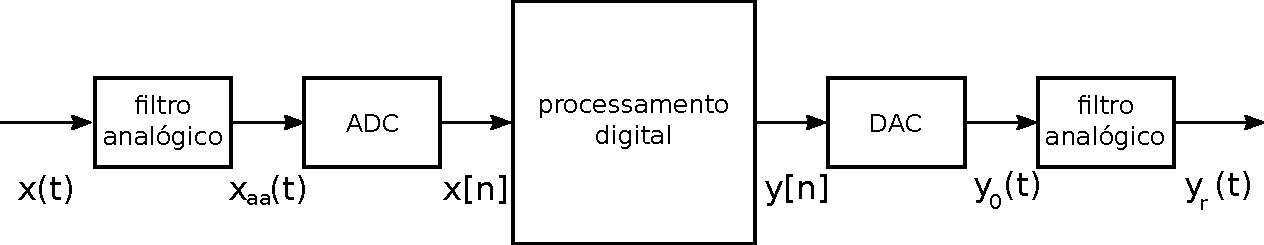
\includegraphics[width=0.7\textwidth]{images/conversaoadda.pdf}
  \caption{Processamento digital de sinais. Conversão AD e DA.}\label{fig-conv-adda}
  \end{figure}

\end{frame}


\begin{frame}%[allowframebreaks]
  \frametitle{Quantização}

  \begin{figure}[h]
  \centering
  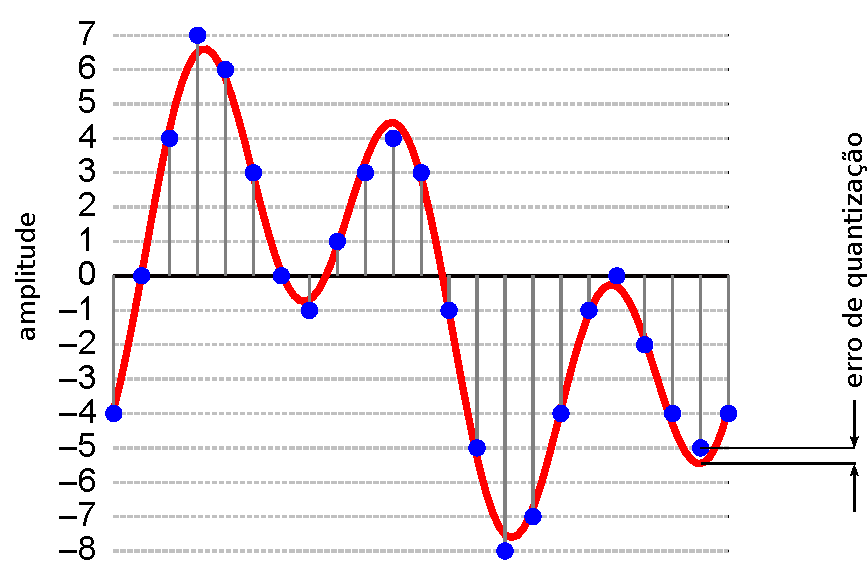
\includegraphics[width=0.5\textwidth]{images/digitalization.pdf}
  \caption{Quantização.}\label{fig-sig-quantz}
  \end{figure}

\end{frame}

\begin{frame}%[allowframebreaks]
  \frametitle{Amostragem}
  Ao amostrar um sinal $x(t)$ com período de amostragem $T_s$ teremos
  \begin{eqnarray}
  x_s(t) &=& x(t) s(t) \nonumber \\ 
        &=& x(t) \sum_{k=-\infty}^{\infty} \delta(t - kT_s) \nonumber \\
         &=& \sum_{k=-\infty}^{\infty} x(kT_s) \delta(t - kT_s)
  \end{eqnarray}

\end{frame}


\begin{frame}%[allowframebreaks]
  \frametitle{Amostragem}

  \begin{figure}[h]
  \centering
  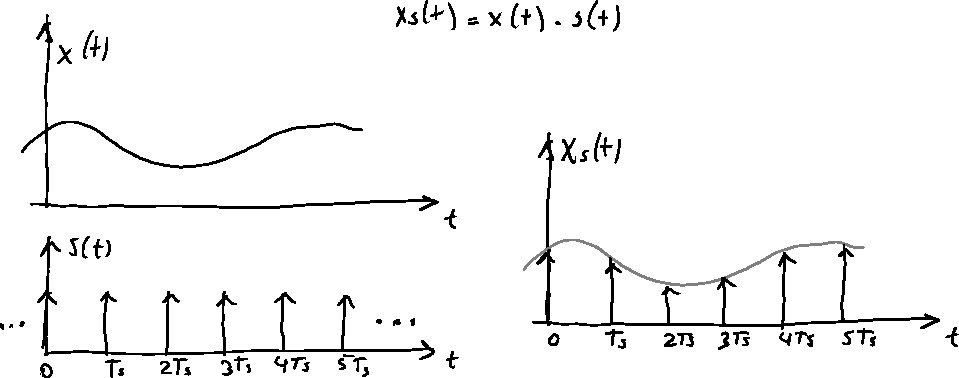
\includegraphics[width=0.8\textwidth]{images/amostragem.pdf}
  %\caption{.}
  \label{fig-amostragem}
  \end{figure}

\end{frame}

\begin{frame}[allowframebreaks]
  \frametitle{Amostragem}
  Como $s(t) = \sum_{k=-\infty}^{\infty} \delta(t - kT_s)$ é periódico com período $T_s$,
  podemos representá-lo por uma série de Fourier:
  \begin{equation}
  s(t) = \sum_{k=\infty}^{\infty} \delta(t - kT_s) = \sum_{k=-\infty}^{\infty} c_k e^{j 2 \pi t k /T_s} \textmd{,}
  \end{equation}
  onde
  \begin{equation}
  c_k = \frac{1}{T_s} \int_{-T_s/2}^{T_s/2} \delta(t) e^{-j2\pi t k/T_s} dt = \frac{1}{T_s}
  \end{equation}
  Desta forma, $x_s(t) = x(t) \cdot s(t)$ poderá ser expresso por
  \begin{equation}
  x_s(t) = \frac{1}{T_s} \sum_{k=-\infty}^{\infty} x(t) e^{j2\pi tk /T_s} \textmd{.}
  \end{equation}

  A multiplicação por $\exp(j 2\pi \alpha t)$ corresponde, na frequência, a um deslocamento de $\alpha$. 
  Teremos assim
  \begin{equation}\label{eq-Xs-freqdom}
  X_s(j \Omega) = \frac{1}{T_s} \sum_{k=-\infty}^{\infty} X \left( j (\Omega - n \Omega_s) \right)
  \end{equation}

  
  \framebreak

  Podemos chegar ao mesmo resultado sabendo que, se no domínio do tempo temos $x_s(t) = x(t) \cdot s(t)$, 
  no domínio da frequência temos
  \begin{equation}\label{eq-conv-dom-freq}
  X_s(j \Omega) = \frac{1}{2\pi} X(j \Omega) \ast S(j \Omega) .
  \end{equation} 
  Como a transformada de Fourier de $s(t)$ é
  \begin{equation}\label{eq-pulse-train-freq}
  S(j \Omega) = \frac{2\pi}{T_s} \sum_{k=-\infty}^{\infty} \delta(\Omega - k \Omega_s) ,
  \end{equation}
  onde $\Omega_s = \nicefrac{2\pi}{T}$, então utilizando as \Cref{eq-conv-dom-freq,eq-pulse-train-freq} obtemos \Cref{eq-Xs-freqdom}.

  \framebreak

  Se $x(t)$ for um sinal limitado em frequência ($\Omega_N$ frequência máxima) e
  não havendo \textit{aliasing}, $\Omega_s > 2 \Omega_N$, podemos reconstruir $x(t)$:
  \begin{equation}\label{eq-x-reconstruido}
  X_r(j \Omega) = H_r(j \Omega) X_s(j \Omega)
  \end{equation}
  onde $H_r$ é um filtro passa-baixas ideal com $\Omega_N < \Omega_c < \Omega_s$.

  \begin{equation}
  H_r (j \Omega) = \begin{cases}1 \quad & \textmd{, se \ \ } \vert \Omega \vert \leq \Omega_c,\\ 0 & \mbox{, caso contrário.}\end{cases}
  \end{equation}

  \vspace{2ex}
  (Teorema da Amostragem)

  \vspace{3ex}
  Leitura: Capítulo 4 \bibentry{oppenheim2009}.
\end{frame}



\begin{frame}%[allowframebreaks]
  \frametitle{Amostragem}

  \begin{figure}[h]
  \centering
  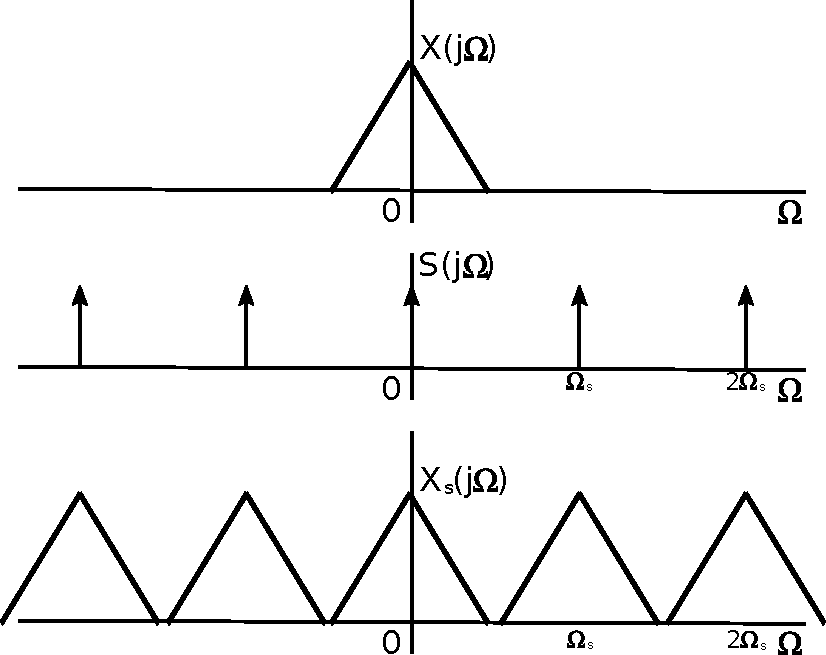
\includegraphics[width=0.6\textwidth]{images/sampling-freq-a.pdf}
  %\caption{.}
  \label{fig-sampling-freq-a}
  \end{figure}

\end{frame}

\begin{frame}%[allowframebreaks]
  \frametitle{Amostragem}

  \begin{figure}[h]
  \centering
  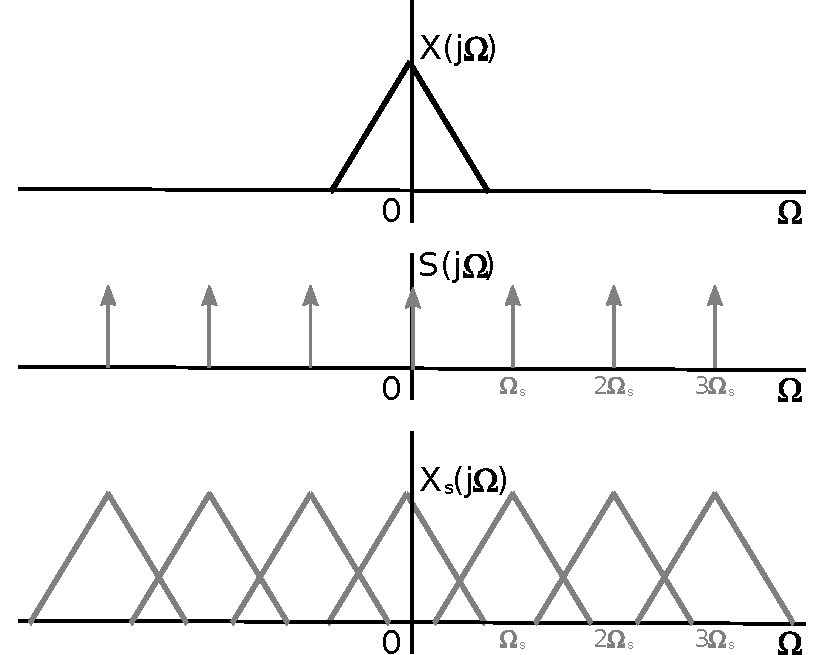
\includegraphics[width=0.6\textwidth]{images/sampling-freq-b.pdf}
  %\caption{.}
  \label{fig-sampling-freq-a}
  \end{figure}

\end{frame}


\subsection{Quantização Escalar}
\begin{frame}[allowframebreaks]
  \frametitle{Quantização Escalar}

  Quantização escalar é um mapeamento $Q$ de valores reais $x$ de uma variável aleatória
  contínua $X$ nos valores $y = Q(x)$, mais próximos de $x$ (em termos de uma determinada medida de distorção),
  de um conjunto discreto e finito $Y = {y_1 , y_2 , \ldots,  y_M }$.
  Os valores $y_i$ , $i = 1, 2, \ldots , M$, são chamados níveis de saída, ou valores de representação,
  ou ainda valores de aproximação. $Y$ é chamado de \textit{codebook} ou conjunto de aproximação.

  \framebreak

  O quantizador escalar é determinado pelo conjunto de limiares 
  $\mathcal{T} = \{t_i\}$, $i=0, 1, \ldots, M$
  e pelo conjunto de pontos de representação $\mathcal{Y} = \{y_i\}$, $i=1, \ldots, M$. 
  Os limiares dividem exaustivamente o domínio $\mathit{R}$ em subintervalos 
  (ou células, regiões de representação) $\Delta_i = (t_{i-1} , t_i ]$ disjuntas,
  ou seja, $\Delta_i \cap \Delta_j = \emptyset$. Diz-se que a divisão é exaustiva
  pois $\bigcup_{i=1}^M \Delta_i = \mathit{R}$. Esta divisão é tal que existe apenas
  um $y_i$ associado a cada intervalo $\Delta_i$, ou seja, $y_i = Q(x)$ se e somente se
  $x \in \Delta_i$. 

  \framebreak 

  \begin{figure}[h!]
  \centering
  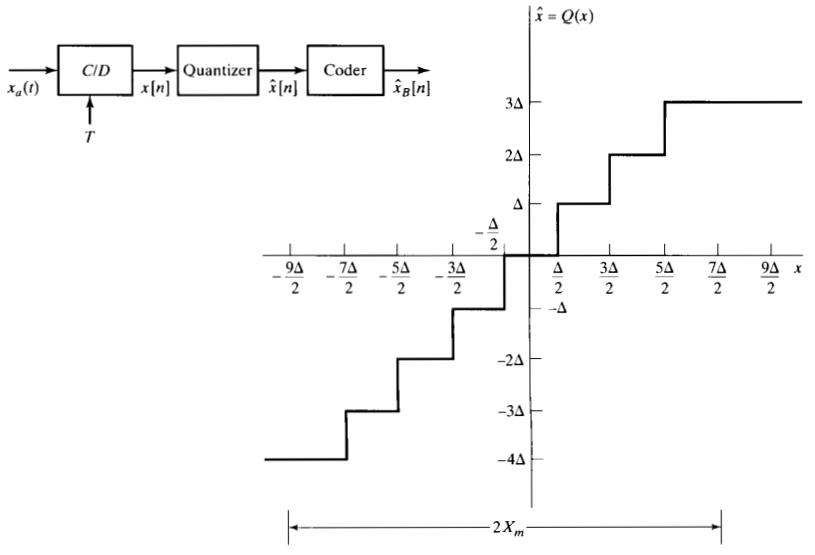
\includegraphics[width=0.6\textwidth]{images/quantization-oppenheim-fig447.png}
  \caption{Quantização. Fonte: \cite{oppenheim2009}.}
  \label{fig:quantization-fig447}
  \end{figure}  

  \framebreak

  É inerente ao processo de quantização a introdução de um erro, chamado \textit{erro de quantização}
  ou \textit{ruído de quantização}.

  O erro de quantização esperado é dado por
  \begin{equation}
  D(Q) = E\left\lbrace d(x,Q(x)) \right\rbrace ,
  \end{equation}
  onde $d(x,Q(x))$ é uma medida de distorção entre $x$ e $Q(x)$, dada por $d(\cdot)$.

  A taxa de quantização é o número de bits $R$ que é utilizado na representação de um valor $x$.
  Ela é dada em bits por amostra.

  Para um quantizador com taxa fixa temos $R = \log_2 M$ bits por amostra.

  \framebreak

  \begin{figure}[h!]
  \centering
  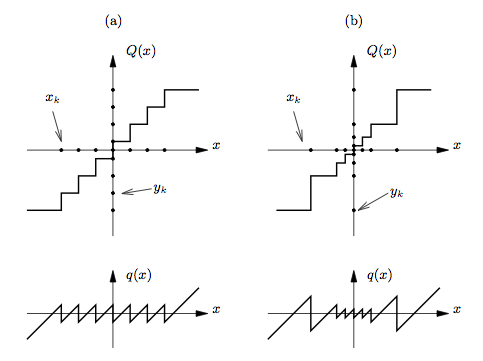
\includegraphics[width=0.55\textwidth]{/home/leoca/ee/ufsj/2012_01/audio_video/aulas/images/quantizationerror.png}
  \caption{(a) linear (b) logarítmico. Fonte: \cite{oppenheim2009}.}
  \label{fig:quantizationerror}
  \end{figure}  

\end{frame}

\subsection{Entropia na saída do quantizador}
\begin{frame}[allowframebreaks]
  \frametitle{Entropia na saída do quantizador}
  As probabilidades dos níveis de representação de um quantizador podem ser determinadas,
  conhecendo-se a pdf do sinal.

  Seja $f(x)$ a pdf (função densidade de probabilidade) de $X$. Podemos calcular a probabilidade
  do i-ésimo nível de reprodução (a probabilidade de $x \in \Delta_i$) como
  \begin{equation}
  P(y_i) = \int_{t_i -1}^{t_i} f(x) \mathrm{d}x .
  \end{equation}
  A entropia da saída do quantizador é igual a
  \begin{equation}
  H(Y) = - \sum_{i=1}^{M} P(y_i) \log_2 P(y_i) .
  \end{equation}

  Um código de comprimento variável poder ser utilizado para representar a saída 
  do quantizador (exemplo: código de Shannon, código Huffman, ou codificação aritmética).
\end{frame}
\note{
Shannon: o limite de representação é a entropia.

O limite para se representar um sinal, sem perdas, será dado pela entropia da fonte.
}


\subsection{Quantização Escalar Uniforme}
\begin{frame}[allowframebreaks]
   \frametitle{Quantização escalar uniforme}
  A quantização escalar é uniforme quando os limiares estão igualmente espaçados,
  e desta forma, as células possuem o mesmo tamanho (exceto as extremas, primeira e última),
  ou seja, $\vert \Delta_i \vert = \delta$, e o ponto de representação localiza-se no 
  ponto médio da célula,
  \begin{equation}
  y_i = \frac{t_{i-1} + t_i}{2} = t_{i-1} + \frac{\delta}{2} , \ \ i=1,2,\ldots,M .
  \end{equation}

  \framebreak

  (*obs.: considerando apenas valores positivos)

  Dada a entrada $x$, a célula associada a $x$ é determinada por
  \begin{equation}
  i = [x / \delta ] ,
  \end{equation}
  onde $\delta$ é a largura de cada célula e $[ \cdot ]$ representa a operação
  de arredondamento.
 
  O valor de aproximação para a entrada $x$ é dado por
  \begin{equation}
  y = Q(x) = \delta \left[ \frac{x}{\delta} \right]   
  \end{equation}
  isto é, a i-ésima célula é determinada por $\Delta_i = (i\delta - \delta/2, i\delta + \delta/2]$
  e $y_i = i\delta$.

\end{frame}

\begin{frame}%[allowframebreaks]
   \frametitle{Distorção no quantizador escalar uniforme}
  Se $f(x)$ é conhecida, então podemos calcular a distorção esperada do quantizador
  \begin{equation}
  D(Q) = \int_{-\infty}^{\infty} f(x) d(x,Q(x)) dx = \sum_i \int_{t_{i-1}}^{t_i} f(x) d(x,y_i) \mathrm{d}x .
  \end{equation}

  Se o erro de distorção é medido pelo erro quadrático, então $D(Q)$ fornecerá o 
  erro quadrático médio (MSE, \textit{Mean Squared Error}):
  \begin{equation}
  D(Q) = \sum_i \int_{t_{i-1}}^{t_i} f(x) (x - y_i)^2 \mathrm{d}x .
  \end{equation}
\end{frame}




\subsection{Quantização Escalar Não-Uniforme}

\begin{frame}[allowframebreaks]
   \frametitle{Quantização escalar não-uniforme}
 
  Se conhecemos as características estatísticas de $X$, podemos utilizar esta informação
  para melhorar as características do quantizador.

  \begin{figure}[h!]
  \centering
  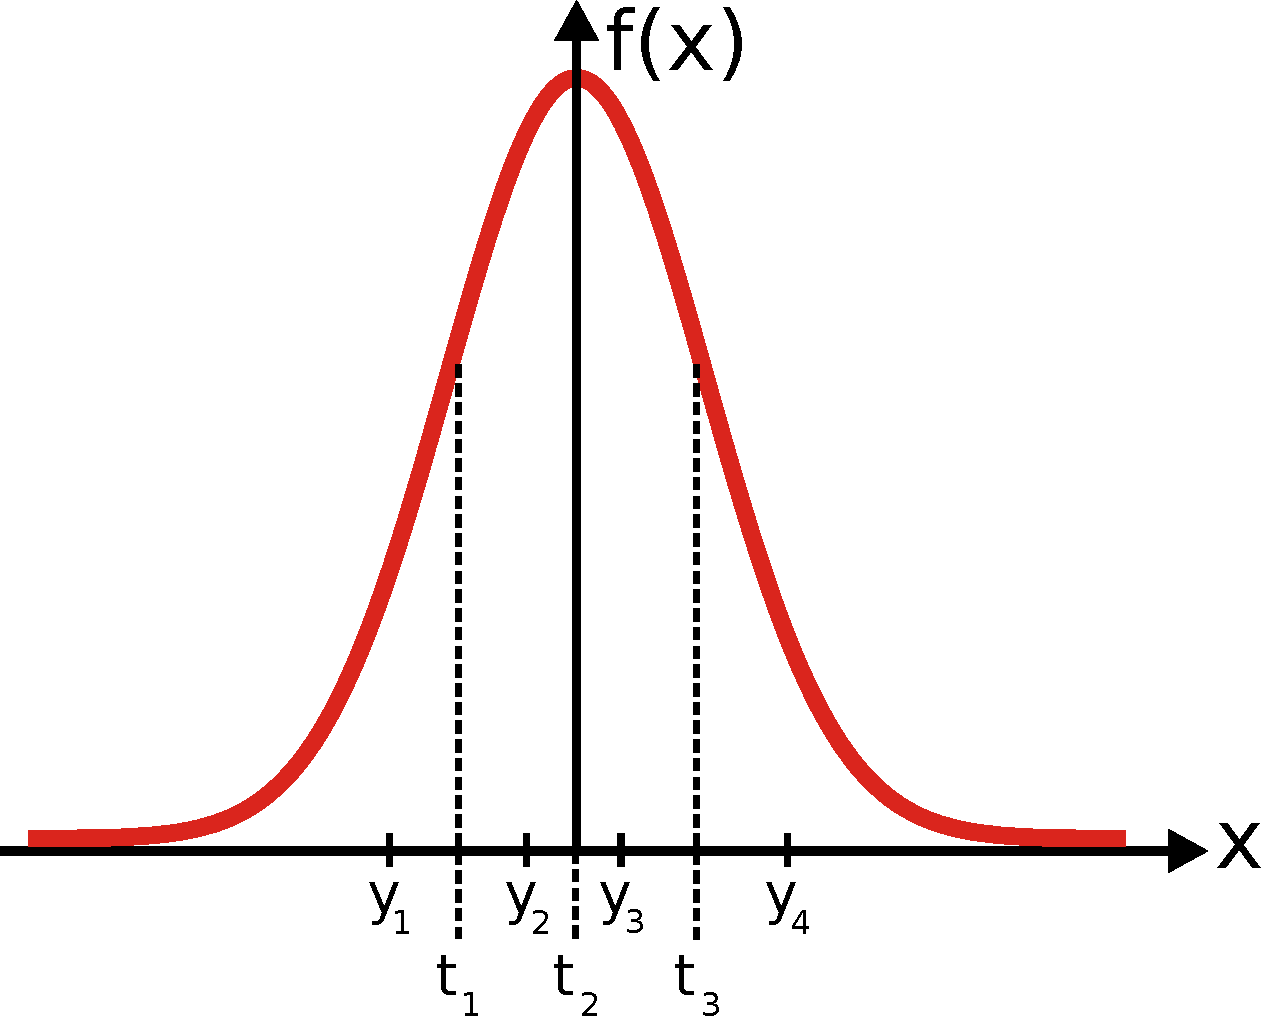
\includegraphics[width=0.45\textwidth]{images/quantz-gaussian.pdf}
  %\caption{}
  \label{fig:quantz-gaussian}
  \end{figure}  
\end{frame}



\subsection{Lloyd-Max}
\begin{frame}[allowframebreaks]
  \frametitle{Algoritmo de Lloyd-Max}
  O algoritmo de \emph{Lloyd-Max} é um algoritmo para encontrar os limiares $\{t_i\}$ e
  os pontos de representação $\{y_i\}$ que minimizam a distorção.

  Lloyd e Max criaram um procedimento para construir uma solução para o problema, que satisfaz
  as condições necessárias (mas não suficientes):

  \begin{itemize}
  \item os limiares devem ficar entre os pontos de representação:
        \begin{equation}
        t_i = \frac{y_{i+1} + y_{i}}{2} \quad , 1 \leq i \leq M-1 , 
        \end{equation}
  \item os pontos de representação devem ficar no meio (com relação à esperança) de um dado intervalo
        \begin{equation}
        y_i = E [ X(i) ] = \frac{ \int_{t_{i-1}}^{t_i} x f_X (x) dx }{ \int_{t_{i-1}}^{t_i} f_X (x) dx  } .
        \end{equation}
  \end{itemize}

  \framebreak
  Algoritmo:
  \begin{enumerate}
  \item Escolher um conjunto inicial arbitrário com $M$ pontos de representação $y_1 < y_2 < \ldots y_M$.
  \item Para cada $i$, $1 \leq j \leq M-1$, fazer $t_i = \frac{1}{2} (y_{i+1} + y_i)$.
  \item Para cada $i$, $1 \leq j \leq M-1$, fazer $y_i$ igual à média condicional de $X \sim f(x)$,
        dado $X \in (t_{i-1}, t_i]$ (onde $t_0$ e $t_M$ são respectivamente $-\infty$ e $+\infty$).
  \item Repetir os passos (2) e (3) até que a melhoria no MSE seja desprezível; então interromper.
  \end{enumerate}
  O MSE decresce (ou permanece o mesmo) a cada passo do algoritmo. Como o MSE é não-negativo,
  ele irá se aproximar de um limite em um número finito de passos, pois o algoritmo será interrompido
  quando a melhoria no MSE foi menor que um dado $\epsilon > 0$.

  \framebreak
  O exemplo abaixo ilustra que o algoritmo deve chegar a um mínimo local.
  Considere $M=2$ pontos de representação e uma pdf $f(x)$ como definida na Figura \ref{fig:lloyd-ex}.

  \begin{figure}[h!]
  \centering
  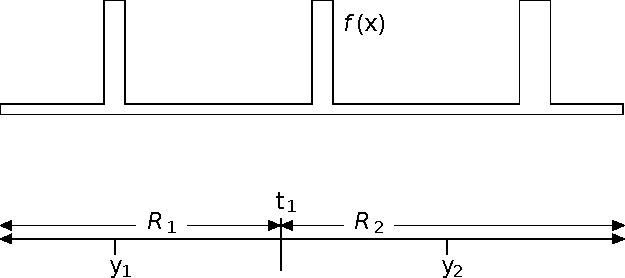
\includegraphics[width=0.55\textwidth]{images/lloyd-ex.pdf}
  \caption{Exemplo Lloyd-Max: regiões e pontos de representação que satisfazem 
        a condição de parada do algoritmo nas não minimizam a distorção média quadrática.
	Fonte: \citet{gallager2008}}
  \label{fig:lloyd-ex}
  \end{figure}

  \framebreak

  A configuração apresentada na Figura \ref{fig:lloyd-ex} satisfaz os critérios de parada, entretanto
  o pico mais a direita é mais provável que os outros dois, desta forma, o MSE poderia ser menor se 
  $R_1$ cobrisse a regiões dos dois picos à esquerda e $R_2$ apenas o pico à direita.

  \vspace{2ex}
  Leitura: Capítulo 3 \bibentry{gallager2008}.
\end{frame}






